\let\negmedspace\undefined
\let\negthickspace\undefined
\documentclass[journal]{IEEEtran}
\usepackage[a5paper, margin=10mm, onecolumn]{geometry}
\usepackage{tfrupee} % Include tfrupee package

\setlength{\headheight}{1cm} % Set the height of the header box
\setlength{\headsep}{0mm}     % Set the distance between the header box and the top of the text

\usepackage{cite}
\usepackage{amsmath,amssymb,amsfonts,amsthm}
\usepackage{graphicx}
\usepackage{textcomp}
\usepackage{xcolor}
\usepackage{listings}
\usepackage{enumitem}
\usepackage{mathtools}
\usepackage{gensymb}
\usepackage{comment}
\usepackage[breaklinks=true]{hyperref}
\usepackage{circuitikz}

\begin{document}

\bibliographystyle{IEEEtran}
\vspace{3cm}

\title{11.16.3.17.3}
\author{EE24BTECH11010 - Balaji B }

{\let\newpage\relax\maketitle}

\renewcommand{\thefigure}{\theenumi}
\renewcommand{\thetable}{\theenumi}
\setlength{\intextsep}{10pt} % Space between text and floats

\numberwithin{equation}{enumi}
\numberwithin{figure}{enumi}
\renewcommand{\thetable}{\theenumi}

If $A$ and $B$ are events such that $P(A)= 0.42$, $P(B)= 0.48$ and $P(A \cap B)= 0.16$, find 
\begin{itemize}
    \item [i)] $P(A \cup B)$
\end{itemize}
\textbf{Solution: }\\
\textbf{Theoretical Solution:\\}
For 2 Boolean variables $A$ and $B$, the axioms of Boolean Algebra are defined as:
\begin{align}
    A + A^\prime &= 1\\
    A + A &= A\\
    AB &= BA\\
    A + B &= B + A\\
    AA^\prime &= 0\\
    P(1) &= 1\\
    P(A + B) &= P(A) + P(B), \text{ if } P(AB) = 0
\end{align}
Using these axioms, we will try to prove that
\begin{align}
    P(A + B) = P(A) + P(B) - P(AB)
\end{align}
We will start by representing $A$ and $B$ as:
\begin{align}
    A &= AB + AB^\prime\\
    B &= AB + A^\prime B\\
    P(A) &= P(AB) + P(AB^\prime)\\
    P(B) &= P(AB) + P(A^\prime B)
\end{align}
On adding \((12)\) and \((13)\),
\begin{align}
A + B &= AB + AB + AB^\prime + A^\prime B\\
    A + B &= AB + AB^\prime + A^\prime B\\
    P(A + B) &= P(AB + AB^\prime + A^\prime B)\\
    P(A + B) &= P(AB) + P(AB^\prime) + P(A^\prime B)\\
    P(A + B) &= P(AB) + P(A) - P(AB) + P(B) - P(AB)\\
    \implies P(A + B) &= P(A) + P(B) - P(AB)
\end{align}
Using the given values of \(P(A), P(B)\) and \(P(AB)\),
\begin{align}
    P(A + B) &= 0.42 + 0.48 - 0.16\\
    P(A + B) &= 0.74
\end{align}
Therefore, the value of \(P(A + B)\) is \(0.74\). \\

\textbf{Computational Solution:}\\
Let \(X_1\) be an indicator random variable of the event \(A\).\\
\(X_1\) is defined as:
\begin{align}
	X_1 =
	\begin{cases}
		1 ,& A\\
		0 ,& A^\prime\\
	\end{cases}
\end{align}
Let \(X_2\) be the indicator random variable of the event \(B\).\\
\(X_2\) is defined as:
\begin{align}
	X_2 =
	\begin{cases}
		1 ,& B\\
		0 ,& B^\prime\\
	\end{cases}
\end{align}
Let \(X_3\) be the indicator random variable of the event \(AB\).\\
\(X_3\) is defined as:
\begin{align}
	X_3 =
	\begin{cases}
		1 ,& AB\\
		0 ,& (AB)^\prime\\
	\end{cases}
\end{align}
The PMF of the random variable \(X_1\) is:
\begin{align}
	p_{X_1}(n) =
	\begin{cases}
		p_1 ,& n = 1\\
		1 - p_1 ,& n = 0
	\end{cases}
\end{align}
The PMF of the random variable \(X_2\) is:
\begin{align}
	p_{X_2}(n) =
	\begin{cases}
		p_2 ,& n = 1\\
		1 - p_2 ,& n = 0
	\end{cases}
\end{align}
The PMF of the random variable \(X_3\) is:
\begin{align}
	p_{X_3}(n) =
	\begin{cases}
		p_3 ,& n = 1\\
		1 - p_3 ,& n = 0
	\end{cases}
\end{align}
where,
\begin{align}
	p_1 &= 0.42\\
	p_2 &= 0.48\\
	p_3 &= 0.16\\
\end{align}
Let \(Y\) be the random variable which is defined as follows:
\begin{align}
	Y = X_1 + X_2 - X_3
\end{align}
But we know that \(X_3\) can never be 0 when \(X_1\) and \(X_2\) are 1 and vice versa.\\
So, \(Y\) is another indicator random variable whose PMF is defined as:
\begin{align}
	p_Y(n) =
	\begin{cases}
		p ,& n = 1\\
		1 - p ,& n = 0
	\end{cases}
\end{align}
\begin{align}
	E(Y) &= E(X_1 + X_2 - X_3)\\
	E(Y) &= E(X_1) + E(X_2) - E(X_3)\\
	1.(p) + 0.(1 - p) &= 1.(p_1) + 0.(1 - p_1) + 1.(p_2) + 0.(1 - p_2) - 1.(p_3) - 0.(1 - p_3)\\
	p &= p_1 + p_2 - p_3
\end{align}
Through our definition, we know that,
\begin{align}
	P(A) &= p_1\\
	P(B) &= p_2\\
	P(AB) &= p_3
\end{align}
Therefore, by comparison of the axiom
\begin{align}
	P(A + B) = P(A) + P(B) - P(AB)
\end{align}
and the equation \((39)\),
\begin{align}
	p &= P(A + B)\\
	P(A + B) &= 0.48 + 0.42 - 0.16\\
	\implies P(A + B) &= 0.74
\end{align}
\begin{figure}[h]
\centering
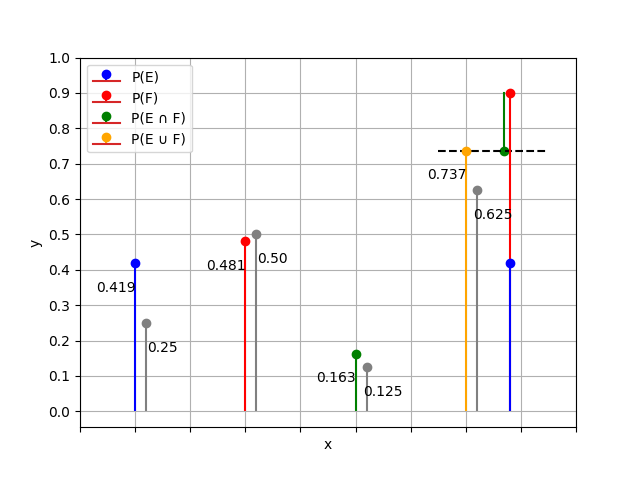
\includegraphics[width=\columnwidth]{figs/Figure_1.png}
\end{figure}
\end{document}
